
%% ==========================================================
This chapter introduces the different implementations done to improve the relevance of the search results,
in addition to the tests concluded to measure the effect that the implementation had.
The purpose of the implementations was to provide a general direction for future development 
while providing some robust data on the performance of the current search application for the organization.
Furthermore, the prerequisite for developing the methods was if one were to succeed over the current
process, the organization would put more effort into developing that method further.



%% ==========================================================
\section{Implementing a relevant search}


The purpose of this section is to introduce how the relevant search was implemented in this thesis.
First, the section provides an overview of the interpretation of how to achieve more relevant search 
results.
Second, the section introduces the methods that were used in creating tokens while indexing.
Lastly, the section describes how the popularity data was collected to replace
the manual process of uploading the score boost, before moving on to introduce
the new ranking function was developed and how the score calculation implemented functioned.


Since relevance is subjective and personalized search was out of scope, as previously mentioned,
a general solution that tried to capture the general relevance of the search results.
Therefore, the purpose was not to show different search results based on the customer who is interacting
with the search application or based on the previous products the customer has viewed.
The solution that was developed by the following parts did not take into account any personalized
information; instead, it tried to achieve good relevance by using the popularity data for products.



%% ==========================================================
\subsection{Creating tokens from content}
\label{ss:methodsTokens}


The following part describes the process of generating tokens from the content of the products.
As previously mentioned, the token generation is a crucial part of a search engine, which indeed became
apparent during the development phase.
Furthermore, during development, there were a few different options tested and considered, the following
part goes through the process of choosing the best one based on the empirical tests concluded 
during development.


The development was done on the Finnish website, where the contents of the products are in Finnish.
Due to the nature of Finnish language having many inflected forms of words, 
it quickly became apparent that only the language analyzer.
Furthermore, this was a case mentioned previously, where the language analyzer could not interpret the meaning
from the words and, while generating good enough tokens for most cases, failed to do so with longer words.
Thus, the first thing where the development started was to investigate how more meaningful tokens could 
be generated.


Since the development was done in Finnish and Elasticsearch supports custom plugins, a new Finnish analyzer 
was found that could solve the problems since it seemed to capture the meaning from even more difficult words well.
However, the decision to not use it was done, since, first, 
it would have required the be installed in the existing production Elasticsearch cluster, and second, 
the language analyzer was only for Finnish, so other Nordic languages would need to use a different solution.
Furthermore, the lack of knowledge about the nuances of other Nordic languages made it impossible to determine
how well the language analyzers were performing in practice.


However, by looking at how the language analyzer worked at a lower level, it became clear that an edge-N-gram analyzer
could be utilized to achieve similar behavior as the language analyzer.
In addition to the similar behavior, the edge-N-gram could capture the meaning from a word better
as the amount of N-grams that were generated could be controlled.
However, capturing meaning from the words did not equal to generating tokens with a minimum length of two, as 
quickly became clear during development.


In addition, a similar problem arose during the usage of an analyzer during search time since if one of the
N-grams generated matched a token in the inverted index, the document was considered a match.
While this is the expected and wanted result, it meant that when generating small N-grams, the precision
of the search results suffered greatly while the recall went up.
The low precision can be observed in Listing \ref{lst:puNGram}, by generating edge-N-grams with a minimum length of two from
the words ``puhelimet`` and ``punainen``.
\begin{lstlisting}[
caption={Output from the edge-N-gram analyzer with a minimum length of two.},
captionpos=b,
label={lst:puNGram},
frame=single]
    [ pu, puh, puhe, puhel, puheli, puhelim, ... ]
    [ pu, pun, puna, punai, punain, punaine, ... ]
\end{lstlisting}
As the first term translates to \emph{phones} and the second term to \emph{red}, the words mean entirely different things,
so by querying either should not match to the other one.


To solve similar problems, as introduced above, a custom edge-N-gram analyzer was created, 
as shown in Figure \ref{fig:new-analyzer}.
Furthermore, the custom analyzer includes two different edge-N-gram analyzers, the first, \emph{edge\_ngram\_analyzer},
which is used during indexing of the documents, and the second, \emph{search\_term\_over\_6}, which is used
during search time.
Both analyzers utilize the same tokenizers and the first two token filters to keep the generated tokens consistent,
first by converting the words to lowercase and then converting them to ASCII characters.


Then, the index time analyzer creates N-grams with a minimum token length of two and a maximum token length of 15 to try
to capture as much meaning from the words as possible.
While, the search time analyzer uses a conditional token filter, which determines if an N-gram should be created or not.
Since the problem in Listing \ref{lst:puNGram}, the search time tokenizer only generates N-grams if the 
search term is over six characters long.
The threshold of six letters was achieved by calculating the average length from the queried search terms over one month.
In addition, six letters seemed to capture the meaning from the words during development well enough that it was chosen.
However, in future development, the process of choosing the threshold could be automated to find the optimal threshold
while balancing precision and recall of the search results.

\begin{figure}
    \centering
    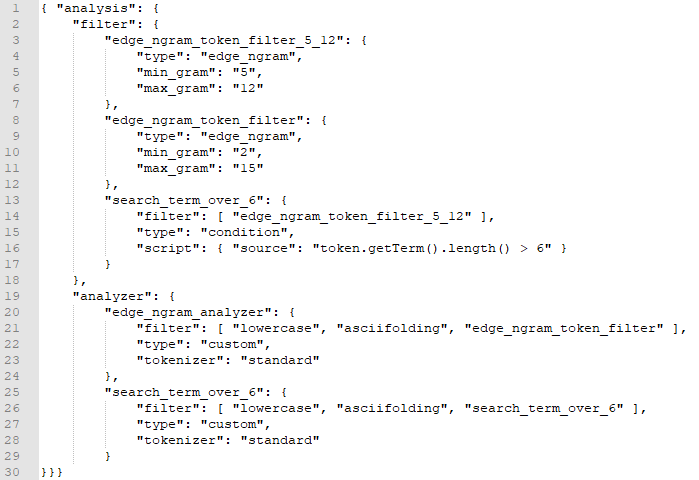
\includegraphics[width=\textwidth]{img/new-analyzer.png}
    \caption{Different analyzers for index time and search time.}
    \label{fig:new-analyzer}
\end{figure}

In summary, by using different analyzers during index time and search time allowed to create shorter N-grams to allow
matching with shorter search terms. 
In addition, the usage of an edge-N-gram analyzer in search time only when the search term exceeded the configured
threshold allowed the exact matching of the shorter search terms.
Furthermore, for longer search terms, the analyzer tried to capture the meaning of the terms and 
match the generated tokens to the inverted index.


The previous part introduced how the text analysis tools provided by Elasticsearch 
were utilized to try to generate meaningful tokens.
In addition, a customer edge-N-gram analyzer was introduced to generate different tokens during indexing and searching.
The following part continues to introduce how the manual process was replaced by an automatic one.


%% ==========================================================
\subsection{Replacing the manual score boosts}


As precious stated, a more general solution was needed, so the purpose of this part is to
introduce how the manual process of updating the score boosts was replaced by an automated process.
As the purpose was not to create separate search strategies based on, for instance, the behavior of a customer, 
a precalculated boost value as the current solution had was enough.
Furthermore, the current solution used many parameters when calculating a new boost value for a product, and 
most of them seemed unnecessary and had little to do with relevance.

So, to answer the question, what customers see relevant, a popularity rating was introduced. 
Furthermore, the rating just included a normalized value of the number of product page views from the previous few days.
However, since the data was not available during indexing, but was collected and stored by Google Analytics,
a new integration was required to import the data.
Thus, a new task was created which imports the data every morning from the previous day and saves the value
to persistent storage, where then the indexing process could fetch the data and calculate the value for the boost.


Calculating data based on the previous days might not be the most accurate at least in e-commerce since 
many factors affect the popularity of a product from different trends to many campaigns and promotions.
So, to keep the rating as updated as possible, a custom function, shown in Figure \ref{fig:new-boost-rating}, was introduced.
Furthermore, the function receives an ordered list of the number of views and weight as input, and then it
calculates the decaying average starting from the first item on the list.
The function weighs the items at the start of the input less than the last items, so this allows the newer 
product page views to affect the resulting rating more than the older dates.


In addition, after calculating the decaying average, the function uses a natural logarithm to flatten the products with
a very high number of views.
Furthermore, a very high view count is not that meaningful since it might negatively affect the ranking, as 
it might override the content score altogether, and it does not capture the popularity that much.
For instance, saying that a product with 10000 views is ten times more popular as a product with 1000 views might not be accurate.
The last step of the score calculation is to normalize the rating, given by the function, across all products
to a value between zero and one.
Furthermore, this prevents high business scores, which might cause the content score to lose meaning in 
the ranking functions.

\begin{figure}
    \centering
    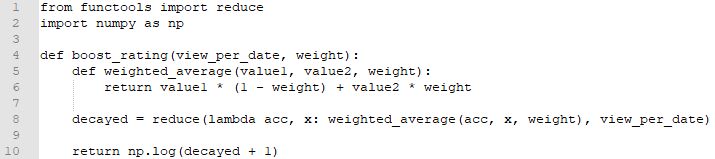
\includegraphics[width=\textwidth]{img/new-boost-rating.png}
    \caption{Function to calculate boost rating based on the number of views.}
    \label{fig:new-boost-rating}
\end{figure}


The previous part introduced the new process introduced to replace the current manual process altogether.
The process included an integration to import data about the number of product page views to the persistent
storage and the number of views to be used to calculate a rating for the products in the index.
The following part continues to introduce how the previous rating is utilized in the ranking algorithm,
which determines the position of the products in the search results.


%% ==========================================================
\subsection{Ranking algorithm}
\label{ss:methodsRanking}

The purpose of this section is to introduce the ranking algorithm used in the implementations.
In total, there were two different ranking algorithms created for this thesis, both utilizing the
calculated popularity rating, introduced in the previous section.
This section will introduce both algorithms and provide the reasoning for developing the first
one further.


The precalculated popularity rating serves as the base for the ranking algorithms.
Furthermore, the first iteration of the ranking algorithm only used the popularity rating 
as the business score.
However, after the first test concluded, it became clear that it did not perform as expected
since the conversion rate went down.
Since the first algorithm did not include anything else other than the popularity score as business scores,
the algorithm captured the intent of users well but did not meet the needs of the business.
Furthermore, the top products in search lists were relevant, but there were multiple cases that the product 
was not in stock.
Thus, providing a relevant search result back to the user, but the search result was still not buyable, 
explaining the drop in conversion rate.


The second algorithm created was similar to the first one with an additional boost if the product was in stock.
The second algorithm uses the following formula to calculate the score for a product
\[ score_{product} = 1 \times score_{popularity} + 0.3 \times score_{stock} + 1 \times score_{content} \]
where the popularity, stock, and content score are first multiplied with weight values, and then 
the sum of all the scores if the calculated score for the product.
The $score_{stock}$ is a value of 1 or 0 depending on if the product has stock and customers can buy it.
The weight values for the individual parameters are a result of the empirical tests and should be a subject
for future development.


The value that changes the most in the ranking algorithms is the content score $score_{content}$.
Furthermore, the base content score is calculated in Elasticsearch by dividing the term frequency with the
inverse document frequency.
However, in this case, the first concluded test showed that the content score calculation in the first algorithm
could be improved since it did not capture exact matches well due to the wildcard nature of the query.

So, the second ranking algorithm, in addition to the updated business score, 
included multiple queries to boost the exact matching results better. 
Furthermore, multiple queries are shown in Figure \ref{fig:new-query}.
Using multiple queries allowed the first query to use wildcard characters both at the start and at the end of 
the search term, the second query to utilize the wildcards at the end of the search term.
The last query did not use any wildcards, so the exact matches received a small boost if they matched 
the third query also.


Elasticsearch allows the usage of multiple queries at the same time withing a \emph{should} clause, so
if a product matches any of the three queries, it will be shown in the search results.
Furthermore, the only difference is if the product matches multiple queries, then the content score
for the product will increase based on how well it matches to the query.
So, each query has a \emph{boost} variable defined, which allows using different weights
for each query. 
As in this setup, the exact queries did not make sense to be boosted highly since while increasing
precision and decreasing recall.
The selected boosts for each of the queries were the result of the empirical tests done during
development.


\begin{figure}
    \centering
    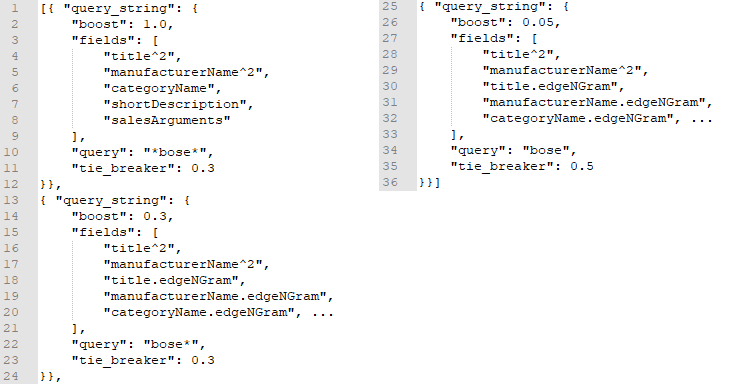
\includegraphics[width=\textwidth]{img/new-query-v.png}
    \caption{Three parallel queries used across different fields.}
    \label{fig:new-query}
\end{figure}


In addition, each of the queries defines a \emph{tie\_breaker} value, which tells Elasticsearch 
that instead of using the \emph{best fields} functionality search across all fields.
Furthermore, the scores from all fields are utilized in the content score calculation, as introduced 
in Section \ref{sec:elasticsearch}.
The utilization of all fields allowed the content score to not only include the best matching field to
reflect the content of the document better.
It seemed to provide better search results during the empirical tests, but in the end, using all
fields depends on the content in the fields.
Furthermore, if the content is very different in the fields, then the usage of only the \emph{best fields}
might be justified.


The previous section introduced different methods for this thesis.
Furthermore, the new methods proposed included new analyzers to generate meaningful tokens, 
the new process to replace the manual process.
In addition to a new ranking function, which utilized the calculate popularity rating for the product
and used multiple queries to manipulate the content score calculation.
The following sections continue to explain how the tests were concluded and how the test results 
were analyzed before the results are introduced.


%% ==========================================================
\section{Testing the search relevance}
\label{sec:methodTests}

The purpose of this section is to introduce the testing methods used and introduce how the test setup worked.
Since the tests were concluded with Google Optimize, which allows running different kinds of tests.
Moreover, in this thesis, simple A/B tests were sufficient enough. 
Google Optimize requires a script to be loaded on page load, and it uses a cookie to determine 
which variant the customer belongs to.

Google Optimize offers a possibility to modify the part of a website while configuring the test, 
which allowed a custom tag to be added when a customer loads the page 
of a website and loads the Google Optimize script.
So by injecting custom HTML tag to the webpage shown to the customer, the front-end JavaScript code could then
determine which variant the customer belonged to and set a custom cookie according to the variant.

When a customer interacted with the search input field and queried something, the receiving back-end
API determined by looking at the cookies of the customer which variant the customer belonged to and constructed the query differently
based on the variant in the cookies.
Furthermore, after constructing the query and posting it through the Query API to the Elasticsearch search engine, 
the results were handled independently of the variant the customer belonged to.
So, only by constructing the query differently based on a cookie value, different results could be shown 
to the customers, by using the same code as before.


While there were four different variants, only one was used by a specific website along with the baseline variant.
Since the tests were concluded in three different websites across Nordic countries, and the codebase is the same
across the website back-ends, there was a need for a total of four variants.
Each variant had different functionality enabled, for instance, the variant \emph{B} had only the new ranking algorithm 
which used the popularity rating and stock availability, and the variant \emph{C} had the new queries for calculating the
content score, but used the old \emph{scoreBoost} field to calculate the business scores.
Furthermore, the variant \emph{D} had both enabled, and the variant \emph{A} was the baseline with nothing new features
enabled.
The specific test setups across the variants are introduced in detail in Section \ref{ch:results}.


This section provided an overview of how the testing setup worked through the third party Google Optimize software.
Furthermore, by creating a cookie to the browser of the customer, the back-end code could construct the Elasticsearch
query differently based on the variant.
The following section introduces how the results from the tests were analyzed before moving on to the actual results.




%% ==========================================================
\section{Analyzing the results}

This section introduces how data from the tests were collected and analyzed using Google Analytics.
Furthermore, Google Analytics is a powerful analytics tool that provides the collection and analysis for organizations.
While Google Analytics collects the data, Google Optimize adds an identifier to the collected data
about what variant the customer has belonged to during the test phase. 
Both products are operated by Google and are used in many organizations across the world.


The measurements introduced in Section \ref{sec:measurements} were used as the primary measurements in this thesis.
However, for a more in-depth analysis of the results, Google Analytics provides a variety of functions to analyze the collected
data.
The measurements were collected based on the time frame of the tests and the identifier added by the Google Optimize.
A more in-depth analysis of the results was not necessary to understand the effects of the concluded tests.
The collected measurements captured the behavior of the customers well, and the result reflects the
expectations moderately.



Since the collected data was cross three different websites, they were easy to differentiate since, for each website, there
is an own Google Analytics project.
The results were collected based on the test version that was concluded, and based on the website, it was concluded in.
The following section will introduce the results in detail and provide an analysis based on the results.